% =======================================================================
\chapter{Motivación}
\label{cap:motivo}
% =======================================================================

\section{Contexto}

Los Problemas de Optimización Combinatoria (POC) aparecen en áreas tan
diversas como la logística, la manufactura, las finanzas y la planificación
de recursos. Su complejidad computacional, mayoritariamente
\NP-dura~\cite{garey1979computers,garey1976complexity}, ha impulsado el
desarrollo de algoritmos exactos y, especialmente, de metaheurísticas capaces
de obtener soluciones de buena calidad en tiempos
prácticos~\cite{gendreau2010handbook}.

La Búsqueda Tabú (\emph{Tabu Search}, TS)~\cite{glover1986future,glover1989tabu,glover1990tabu}
registra los movimientos recientes en una lista tabú para evitar la re-visita
de soluciones y escapar de óptimos locales. Sobre este mecanismo básico se
puede construir una familia completa de refinamientos: memoria de largo plazo,
criterios de aspiración, reinicios informados y penalizaciones
adaptativas~\cite{glover1997tabu}. Cada uno de estos componentes tiene un costo
de implementación y un costo computacional, y la pregunta práctica
—\emph{¿cuánto contribuye realmente cada uno?}— rara vez se responde de forma
aislada.

\section{La brecha que motiva este trabajo}

La literatura sobre Búsqueda Tabú sigue mayoritariamente dos caminos:

\begin{enumerate}
  \item \textbf{Comparación entre familias de metaheurísticas.} Se contrasta
    TS con algoritmos genéticos (GA)~\cite{holland1975adaptation}, recocido
    simulado (SA)~\cite{kirkpatrick1983optimization} u optimización por
    colonias de hormigas (ACO)~\cite{dorigo1996ant}. El resultado informa qué
    familia conviene, pero no qué componentes internos de TS son responsables
    del rendimiento.
  \item \textbf{Variantes altamente especializadas.} Se propone una versión de
    TS finamente ajustada a un único problema~\cite{cordeau2002guide}. El
    resultado es competitivo, pero difícilmente transferible: no se sabe si la
    ganancia proviene del mecanismo o del ajuste al problema.
\end{enumerate}

Existe, entonces, una brecha metodológica: \emph{faltan repositorios públicos
que ilustren la progresión interna de la Búsqueda Tabú} —de una configuración
básica a una avanzada— sobre múltiples problemas heterogéneos, con código
reproducible y métricas comparativas unificadas.

Este trabajo aborda esa brecha con un diseño deliberadamente simple: se fijan
\textbf{tres niveles de TS} y se aplican, sin re-ajustes oportunistas, a
\textbf{cinco problemas} de naturaleza distinta. Entre columnas varía el
mecanismo; entre filas, el problema. La diferencia observada es, por
construcción, atribuible al mecanismo.

\begin{table}[H]
\centering
\caption{Los tres niveles del Triple Enfoque Resolutivo}
\label{tab:niveles}
\small
\begin{tabular}{lp{9cm}}
\toprule
\textbf{Nivel} & \textbf{Mecanismos incorporados} \\
\midrule
TS-Básico      & Lista tabú de tamaño fijo, vecindad simple, aspiración
                 elemental. Sin memoria de largo plazo. \\
TS-Intermedio  & Lista tabú dinámica, criterio de aspiración explícito y
                 reinicio suave ante estancamiento. \\
TS-Avanzado    & Memoria de frecuencia, penalización adaptativa
                 ($\lambda$ variable) y diversificación informada mediante
                 perturbación estructural. \\
\bottomrule
\end{tabular}
\end{table}

\section{Objetivos}
\label{sec:objetivos}

\subsection*{Objetivo general}

Desarrollar un repositorio que cuantifique la contribución incremental de
cada mecanismo de Búsqueda Tabú sobre cinco problemas clásicos de
optimización combinatoria de estructura heterogénea.

\subsection*{Objetivos específicos}

\begin{enumerate}
  \item \textbf{Implementar} quince módulos de Búsqueda Tabú —cinco problemas
    por tres niveles de complejidad— bajo una interfaz uniforme que permita
    tratarlos de forma homogénea, con parámetros fijados por problema y sin
    re-ajuste por instancia.
  \item \textbf{Automatizar} la ejecución y la persistencia de los 360
    experimentos que resultan del diseño factorial, para reproducirlos por
    completo sin intervención manual.
  \item \textbf{Medir} la contribución de cada mecanismo mediante una métrica
    comparable entre problemas de unidades distintas, validada sobre semillas
    independientes para distinguir el efecto real del ruido muestral.
  \item \textbf{Publicar} el repositorio con el código, las instancias, los
    modelos exactos de verificación y los resultados, de forma que un tercero
    pueda reproducir los hallazgos y extender el trabajo a nuevos problemas o
    algoritmos sin modificar la infraestructura existente.
\end{enumerate}

\section{El objeto de estudio: cinco problemas}

Los cinco problemas se eligieron porque cubren estructuras de solución
distintas —selección de subconjuntos~\cite{martello1990knapsack}, permutación
circular~\cite{applegate2006traveling}, partición en
rutas~\cite{toth2002vehicle}, permutación lineal y grafo de
disyunción~\cite{pinedo2016scheduling}— y por lo tanto exigen vecindades y
codificaciones diferentes. Un mecanismo que mejora en los cinco es
plausiblemente un mecanismo general.

\begin{table}[H]
\centering
\caption{Problemas, estructura de solución y vecindad empleada}
\label{tab:problemas}
\small
\begin{tabular}{llll}
\toprule
\textbf{Problema} & \textbf{Estructura} & \textbf{Vecindad} &
  \textbf{Objetivo} \\
\midrule
Knapsack 0/1 & Vector binario     & Flip / swap       & Maximizar valor \\
TSP          & Permutación circular & 2-opt           & Minimizar distancia \\
CVRP         & Partición en rutas & 2-opt intra/inter & Minimizar distancia \\
Flowshop     & Permutación lineal & Swap adyacente    & Minimizar $C_{\max}$ \\
Job Shop     & Grafo disyuntivo   & Swap en ruta crítica & Minimizar $C_{\max}$ \\
\bottomrule
\end{tabular}
\end{table}

\section{El código como argumento}

El repositorio no es un anexo del trabajo: es el trabajo. La afirmación
central —que ciertos mecanismos de memoria explican la mejora— solo es
verificable si el lector puede leer y ejecutar exactamente la medición realizada.
Los fragmentos que siguen muestran dónde vive esa diferencia.

\subsection{Una interfaz, cinco problemas}

Los quince módulos (5~problemas $\times$ 3~niveles) exponen la misma firma y
devuelven el mismo diccionario. Esta homogeneidad permite que un único
orquestador ejecute todo el experimento sin ramificaciones por problema.

\lstinputlisting[caption={Interfaz uniforme de los quince módulos de
Búsqueda Tabú},label={lst:interfaz}]{codigos/01_interfaz_solve.py}

\subsection{Nivel 1: la lista tabú desnuda}

En TS-Básico toda la memoria del algoritmo cabe en una \texttt{deque} de
tamaño fijo: una cola de doble extremo de la biblioteca estándar de Python
que, al llenarse, descarta automáticamente el elemento más antiguo. El criterio de aspiración existe, pero en su forma mínima: un
movimiento prohibido se admite únicamente si mejora el mejor valor global.

\lstinputlisting[caption={Núcleo de TS-Básico para TSP: vecindad 2-opt y
lista tabú de tamaño fijo},label={lst:basico}]{codigos/02_ts_basico_nucleo.py}

\subsection{Nivel 3: memoria de largo plazo}

TS-Avanzado añade tres mecanismos que operan sobre la \emph{historia} de la
búsqueda y no solo sobre las últimas iteraciones. La penalización adaptativa
es el punto clave: el costo de un movimiento se corrige con la frecuencia
histórica de las aristas que elimina; así, la búsqueda se aleja de las
regiones ya recorridas.

\lstinputlisting[caption={TS-Avanzado para TSP: memoria de frecuencia, lista
tabú dinámica, reinicio \emph{double-bridge} y penalización
adaptativa},label={lst:avanzado}]{codigos/03_ts_avanzado_memoria.py}

\subsection{Una sola métrica}

Comparar cinco problemas con unidades incomparables (valor, distancia,
\emph{makespan}) exige normalizar. El GAP porcentual respecto al mejor valor
conocido (BKS) cumple ese papel:

\begin{equation}
  \text{GAP}(\%) =
  \begin{cases}
    \dfrac{f^* - \text{BKS}}{\text{BKS}} \times 100
      & \text{minimización} \\[8pt]
    \dfrac{\text{BKS} - f^*}{\text{BKS}} \times 100
      & \text{maximización}
  \end{cases}
  \label{eq:gap_motivo}
\end{equation}

\lstinputlisting[caption={Cálculo del GAP respecto al
BKS},label={lst:gap}]{codigos/04_metrica_gap.py}

\section{Qué muestran los datos}

Las figuras de este apartado resumen los 360 experimentos y justifican, a
posteriori, el interés del enfoque.

La Figura~\ref{fig:gap_global} muestra el resultado principal: el GAP global
promedio cae de \SI{6.50}{\percent} en TS-Básico a \SI{3.40}{\percent} en
TS-Avanzado, una reducción del \SI{48}{\percent} relativo. El salto mayor
ocurre entre el nivel 1 y el 2; el nivel 3 aporta una mejora adicional más
pequeña pero consistente.

\begin{figure}[H]
  \centering
  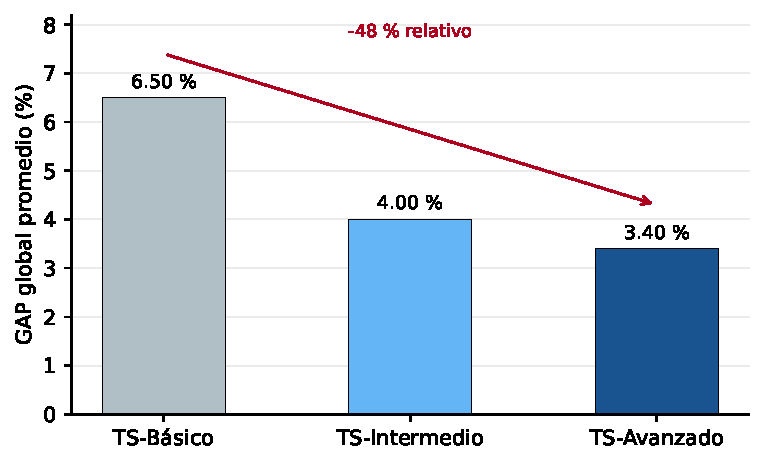
\includegraphics[width=0.72\linewidth]{gap_global.pdf}
  \caption{GAP global promedio por nivel de Búsqueda Tabú sobre los cinco
           problemas (360 experimentos, 5 semillas).}
  \label{fig:gap_global}
\end{figure}

El promedio global, sin embargo, oculta un efecto no uniforme. La
Figura~\ref{fig:gap_problema} desagrega por problema en escala logarítmica:
CVRP concentra casi toda la ganancia (de \SI{19.22}{\percent} a
\SI{6.38}{\percent}), mientras que en Flowshop los tres niveles quedan en
torno al \SI{1.7}{\percent} y la diferencia entre ellos es marginal.

\begin{figure}[H]
  \centering
  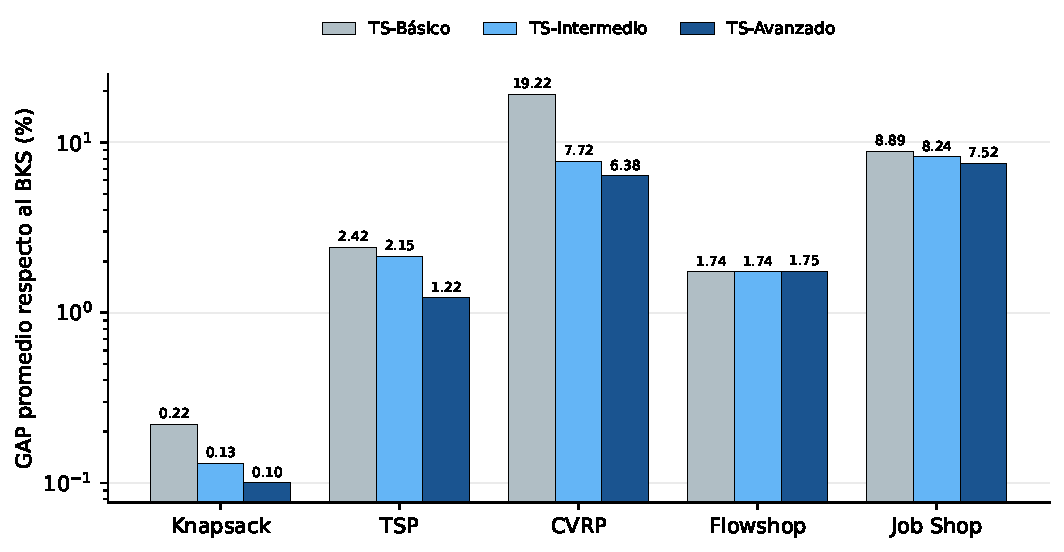
\includegraphics[width=\linewidth]{gap_por_problema.pdf}
  \caption{GAP promedio por problema y nivel (escala logarítmica). El efecto
           de los mecanismos de memoria depende fuertemente del problema.}
  \label{fig:gap_problema}
\end{figure}

Esa heterogeneidad es, en sí misma, un resultado: los mecanismos de memoria
de largo plazo rinden donde el espacio de búsqueda es amplio y accidentado
(CVRP, Job Shop), y aportan poco donde la vecindad deja escaso margen sobre la
solución constructiva (Flowshop con NEH e intercambio adyacente, Knapsack
con \emph{greedy} por ratio).

La mejora no es gratuita. La Figura~\ref{fig:calidad_tiempo} sitúa cada nivel
en el plano calidad--costo: TS-Avanzado requiere aproximadamente
$3.9\times$ el tiempo de TS-Básico para obtener cerca de la mitad del GAP.

\begin{figure}[H]
  \centering
  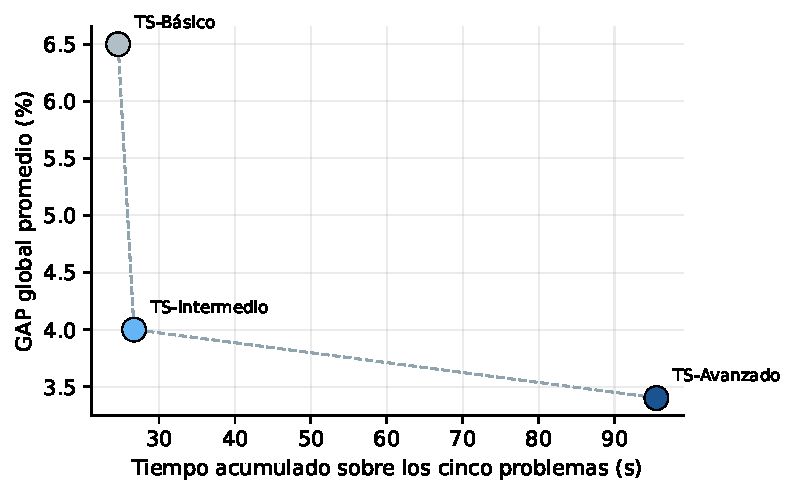
\includegraphics[width=0.72\linewidth]{calidad_vs_tiempo.pdf}
  \caption{Compromiso entre calidad de solución y costo computacional
           acumulado sobre los cinco problemas.}
  \label{fig:calidad_tiempo}
\end{figure}

Finalmente, la Figura~\ref{fig:dispersion} muestra la desviación estándar del
GAP entre las cinco semillas. La baja dispersión en la mayoría de las
instancias respalda que las diferencias observadas entre niveles no son ruido
muestral.

\begin{figure}[H]
  \centering
  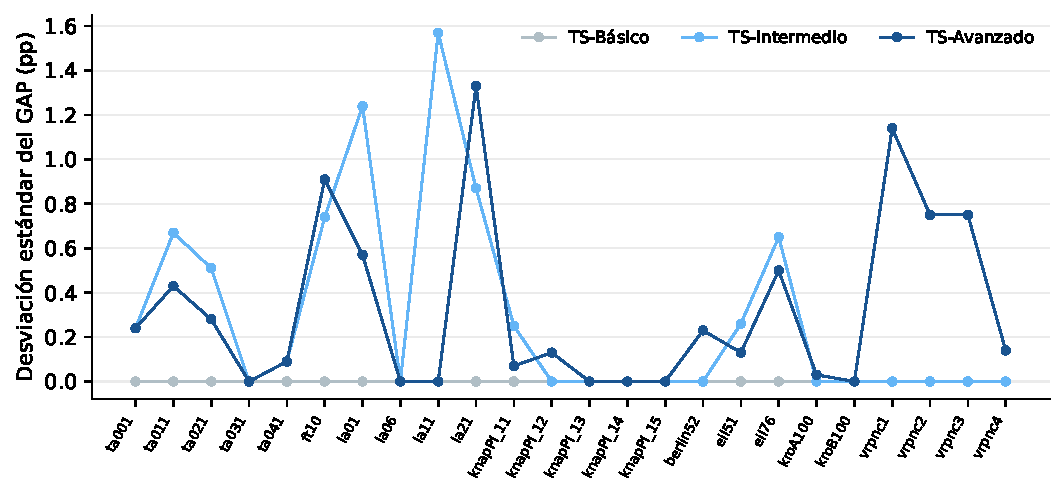
\includegraphics[width=\linewidth]{dispersion_semillas.pdf}
  \caption{Desviación estándar del GAP entre las cinco semillas
           $\{42, 123, 456, 789, 1337\}$, por instancia y nivel.}
  \label{fig:dispersion}
\end{figure}

\section{Contribuciones}

Mientras los objetivos de la Sección~\ref{sec:objetivos} declaran la intención,
esta sección enuncia lo efectivamente obtenido:

\begin{enumerate}
  \item \textbf{Una medición de la contribución de cada mecanismo.} La progresión de
    TS-Básico a TS-Avanzado reduce el GAP global de \SI{6.50}{\percent} a
    \SI{3.40}{\percent}, y el trabajo establece cuánto de esa reducción
    corresponde a cada componente: 2.50 puntos porcentuales a la lista tabú
    dinámica y 0.60 a los mecanismos de memoria de largo plazo.
  \item \textbf{La constatación de un efecto no uniforme.} La ganancia
    se concentra en los problemas de espacio de búsqueda amplio —CVRP reduce
    su GAP un \SI{67}{\percent} relativo— y resulta marginal donde la
    vecindad deja escaso margen sobre la solución constructiva. Esto acota
    cuándo conviene pagar el costo de los mecanismos avanzados.
  \item \textbf{Un criterio de decisión práctico.} TS-Avanzado exige
    aproximadamente $3.9\times$ el tiempo de TS-Básico para obtener cerca de
    la mitad del GAP, mientras TS-Intermedio captura el \SI{81}{\percent} de la mejora
    total a una fracción de ese costo.
  \item \textbf{Un repositorio público y reproducible} con las quince
    implementaciones, el orquestador de los 360 experimentos, modelos exactos
    de verificación y los resultados persistidos, extensible a nuevos
    problemas o algoritmos sin modificar la infraestructura existente.
\end{enumerate}

\section{Estructura del documento}
\label{sec:estructura}

El resto del documento se organiza en cinco capítulos:

\begin{itemize}
  \item El \textbf{Capítulo~\ref{cap:metodologia}} describe la metodología
    de trabajo: el diseño factorial, las decisiones que delimitan el
    estudio, las instancias de prueba, el protocolo experimental y los
    controles de validación.
  \item El \textbf{Capítulo~\ref{cap:paper}} incluye el artículo en formato
    IEEE, con el marco teórico de los cinco problemas, el pseudocódigo de
    los tres niveles de Búsqueda Tabú y los resultados desagregados por
    problema.
  \item El \textbf{Capítulo~\ref{cap:afiche}} presenta el afiche con que el
    trabajo se expuso en EXPOTIC UNAB 2026.
  \item El \textbf{Capítulo~\ref{cap:repositorio}} documenta el repositorio
    desde la ingeniería de software: requisitos, arquitectura, componentes,
    uso y extensión.
  \item El \textbf{Capítulo~\ref{cap:conclusion}} resume los hallazgos, las
    limitaciones y el trabajo futuro.
\end{itemize}
